\documentclass{article}
\usepackage[margin=25mm]{geometry}
\usepackage{amsmath,amsthm,booktabs}
\usepackage[xetex]{xcolor}
\usepackage{tikz}
\usetikzlibrary{arrows.meta}
\usepackage[xetex,colorlinks,linkcolor=blue!60!black,citecolor=green!40!black,urlcolor=blue!60!black]{hyperref}
\usepackage[nameinlink,capitalise]{cleveref}
\newtheorem{proposition}{Proposition}
\title{A small document with a lot to preview}
\author{TeXpresso inside VS Code}
\date{}

\begin{document}
\maketitle
\section{An immediate connection}\label{sec:start}
Edit this sentence and watch the preview change. Use the PNG/SVG/Auto selector
in the toolbar to compare rendering, or hold the magnifier over a detail.
Control or Command click on the page to return to the source.

This example combines mathematics, a TikZ illustration, cross-references with
\texttt{cleveref}, and a bibliography. Follow the links to
\cref{fig:curve,tab:checklist,sec:references}, then return here using
\cref{sec:start}. The citations to \cite{knuth1984,tikz} are links too.

\subsection{From equations to references}
The Gaussian integral gives a useful normalisation:
\begin{equation}\label{eq:gaussian}
  \int_{-\infty}^{\infty} e^{-x^2}\,\mathrm{d}x=\sqrt{\pi}.
\end{equation}
\Cref{eq:gaussian} stays linked when its number changes. Insert another numbered
equation above it to try this. The preview reruns after an editing pause to
resolve references.

\begin{proposition}\label{prop:sum}
For every integer $n\geq1$, $\sum_{k=1}^{n}k=n(n+1)/2$.
\end{proposition}
\begin{proof}
Pair the first and last terms: each pair sums to $n+1$.
Equivalently, add the sum in forward and reverse order and divide by two.
\end{proof}
\Cref{prop:sum} is deliberately simple; the interesting part here is that its
reference, like the equation and figure references, remains clickable.

\medskip
\noindent\hyperref[fig:curve]{Continue to the diagram on the next page}
\hfill\href{https://github.com/let-def/texpresso}{TeXpresso on GitHub}

\newpage
\section{A figure you can change}\label{sec:figure}
The paths in \cref{fig:curve} mix text, filled areas, thin strokes and arrowheads.
Change the two control-point heights below to reshape the curve. Edits inside
the picture also exercise a different compiler workload from prose edits.

% Try changing 2.3 to 1.3, or 0.3 to 1.3, in the control points below.
\begin{figure}[ht]
\centering
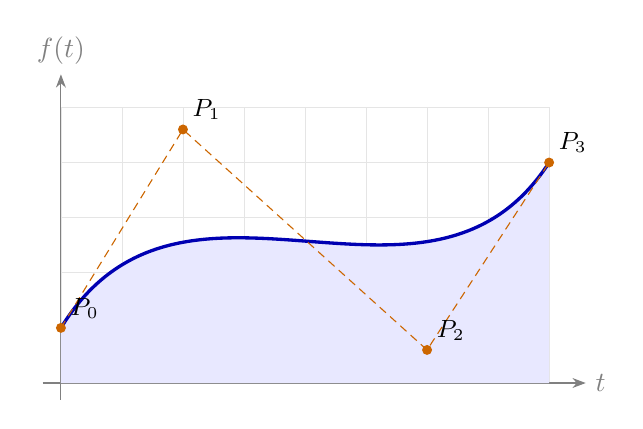
\begin{tikzpicture}[x=1.55cm,y=1.4cm,>=Stealth]
  \draw[step=.5,gray!20,very thin] (0,0) grid (4,2.5);
  \draw[->,gray] (-.15,0) -- (4.3,0) node[right] {$t$};
  \draw[->,gray] (0,-.15) -- (0,2.8) node[above] {$f(t)$};
  \fill[blue!9] (0,0) -- (0,.5)
    .. controls (1,2.3) and (3,0.3) .. (4,2) -- (4,0) -- cycle;
  \draw[blue!70!black,very thick] (0,.5)
    .. controls (1,2.3) and (3,0.3) .. (4,2);
  \draw[densely dashed,orange!80!black] (0,.5) -- (1,2.3) -- (3,.3) -- (4,2);
  \foreach \x/\y/\label in {0/.5/P_0,1/2.3/P_1,3/.3/P_2,4/2/P_3} {
    \fill[orange!80!black] (\x,\y) circle (1.8pt);
    \node[above right,font=\small] at (\x,\y) {$\label$};
  }
\end{tikzpicture}
\caption{A cubic B\'ezier curve with its control polygon. The picture is drawn
from source using TikZ~\cite{tikz}.}\label{fig:curve}
\end{figure}

\begin{table}[ht]
\centering
\begin{tabular}{lll}
\toprule
Feature & Something to try & Reference \\
\midrule
Mathematics & Insert an equation & \cref{eq:gaussian} \\
TikZ & Move a control point & \cref{fig:curve} \\
Cross-references & Insert a proposition & \cref{prop:sum} \\
Bibliography & Follow a citation & \cite{knuth1984} \\
\bottomrule
\end{tabular}
\caption{A few small edits to explore.}\label{tab:checklist}
\end{table}

\noindent\hyperref[sec:start]{Back to the introduction}
\hfill\hyperref[sec:references]{Continue to the bibliography}

\newpage
\section{Reading and references}\label{sec:references}
The bibliography is generated from \texttt{showcase.bib} using BibTeX.
Knuth's account of \TeX~\cite{knuth1984} and the TikZ manual~\cite{tikz}
provide two sample entries. Their citation links jump to the entries below.

The demo launcher runs \texttt{latexmk -xelatex} locally before opening the
preview, so citations and forward references are already resolved.
After changing the bibliography, run
\emph{TeXpresso: External Compile and Refresh} from the Command Palette.
Ordinary source edits and reference updates use TeXpresso's automatic reruns.

\Cref{fig:curve,tab:checklist} are on the previous page;
\cref{eq:gaussian,prop:sum} are on the first. Try following these links with the
magnifier enabled, or use the page controls to navigate back and forth.

\bibliographystyle{plain}
\bibliography{showcase}
\end{document}
